%\documentclass[11pt, oneside]{book}
\documentclass[11pt, twoside]{book}  %importante cambiar si es libro
\usepackage[utf8]{inputenc}
\usepackage[T1]{fontenc}


%%%%%%%%%%%%%%%%%%%%%%%%%%%%%%%%%%%%%%%%%%%%%%%%%%%%%%%%%
%   Paquetes y librerías iniciales para un documento,
%           Graficos, simbolos, tablas, bibliografía
%%%%%%%%%%%%%%%%%%%%%%%%%%%%%%%%%%%%%%%%%%%%%%%%%%%%%%%%%
%---------------------------------------------------------------------------
% Esto es para que el LaTeX sepa que el texto está en español:
\usepackage[spanish,es-noshorthands,es-tabla]{babel}
\selectlanguage{spanish}
%---------------------------------------------------------------------------
% para uso en modo matemático
\usepackage{amssymb}
\usepackage{amsthm}
\usepackage{amsmath}

%---------------------------------------------------------------------------
% Para las imagenes

\usepackage[dvips]{graphicx}
\graphicspath{{Figuras/}} % se fija el camino para las figuras
\usepackage{rotating}  %para poder rotar las figuras
\usepackage{wrapfig}

%---------------------------------------------------------------------------
% PIES DE FOTOS Y TABLAS

\usepackage{float} % para objetos flotantes
\usepackage{caption} % para los pies de fotos o tablas
\usepackage{subcaption}
\captionsetup{font=small,labelfont=bf} % para tamaño y tipo fuentes pie de foto
\usepackage{multirow} % para las tablas unir columnas
\usepackage{multicol} %para escribir en multiples columnas

% Referencias y biblio

\usepackage{pdfpages}
%\usepackage[pdftex,breaklinks=true,hidelinks]{hyperref} % para referencias/indice en pdf

\usepackage[
breaklinks=true,colorlinks=true,
linkcolor=blue,urlcolor=blue,citecolor=blue,% PDF VIEW
linkcolor=black,urlcolor=black,citecolor=black,% PRINT
bookmarks=true,bookmarksopenlevel=2]{hyperref}

\usepackage{emptypage}
\usepackage{ragged2e} %Justificacion

%\usepackage[toc,title,page]{appendix}

%Para bibliografía
\usepackage[numbers,square]{natbib}
\bibliographystyle{apalike}
%\bibliographystyle{IEEEtran}

%%%%%%%%% HAbituales estilos
%plainnat
%%abbrvnat
%unsrtnat  %Items in bibliography sorted in order cited)
%IEEEtran

%

%%%%%%%%%%%%%%%%%%%% Formato de la ual %%%%%%%%%%%%%%%%%%%%%%%%%%%%%%%%%


\usepackage{UAL}
%\usepackage[print,doble]{UAL}
\usepackage{codigo}

%%%%%% PAQUETES INCORPORADOS POR EL USUARIO

\usepackage{longtable}   %Tablas largas
\usepackage{verbatim}
\usepackage{textcomp} %para completar los signos válidos
\usepackage{eurosym} %simbolo del euro [\euro]
\usepackage[bottom]{footmisc}



%%%%%%%%%%%%%%%%%%%%%%%%%%%%%%%%%%%%%%%%%%%%%%%%%%%
% Datos identificativos del TFG                            %
%%%%%%%%%%%%%%%%%%%%%%%%%%%%%%%%%%%%%%%%%%%%%%%%%%%

\author{David Camacho Jurado}
\titulo{Regulación del confort del \textit{smarthome} a partir de una estación meteorológica y sensores ambientales}
\estudios{Grado en Informática}
\universidad{UNIVERSIDAD DE ALMERIA}
\director{Juana López Redondo}
\direct{Marcos Lupión Lorente}
\curso {2021/2022}


\pagestyle{cab}

\begin{document}
\frontmatter

\portada

\begin{dedicatoria}
    Texto de la dedicatoria
\end{dedicatoria}



%%%%%%%%%%%%%%%%%%%%%%%%%%%%%%%%%%%%%%%%%%%%%%%%%%%%%%%%%%%%%%%%%%%%%%%%%%%%
%%%%%%%%%%%%%%% ESTO ES PARA LA TABLA DE CONTENIDOS (INDICE)%%%%%%%%%%%%%%%%


\setcounter{secnumdepth}{3} %niveles en capitulos hasta (1.1.1)
\setcounter{tocdepth}{3} %niveles en indice hasta (1.1)


\addtocontents{toc}{~\hfill\small{Página}\par} %añade "pagina" a tabla de contanidos
\addtocontents{toc}{\vspace{2pt} \hrule \vspace{5mm} \par}

%\renewcommand\contentsname{Índice de contenidos}
\tableofcontents
\listoffigures % indice de figuras
\listoftables % indice de tablas
\lstlistoflistings % indice de listados



%---------------------------------------------------------------------------
% comienzo de relacion abreviaturas y/o acrónimos
%---------------------------------------------------------------------------


%\addcontentsline{toc}{section}{ABREVIATURAS}
\clearpage
\vspace{0.2cm}
\section*{ABREVIATURAS}

\begin{tabular}{ l   |    l  }
	

&\\
   ESI & Escuela Superior de ingeniería \\
   InSo & Ingeniería del Software \\
    SBSE& Search based software engineering\\
   TFG & Trabajo fin de grado\\
   
      UAL & Universidad de Almería \\
      &\\

\end{tabular}


%\addcontentsline{toc}{section}{ABREVIATURAS}



% Borra el bloque si sólo queremos resumen en contraportada
\addcontentsline{toc}{chapter}{Resumen y Abstract}
\chapter*{Resumen y Abstract}

En este archivo se incluirá tanto el resumen en castellano como su traducción al inglés. Los dos párrafos estarán ligeramente separados.

El  propósito  del  trabajo  en  una  o  dos  frases.  El  diseño  y metodología  utilizada,  los  resultados  más  significativos  del trabajo realizado y un breve resumen de las conclusiones. Debe ser conciso y presentar los resultados obtenidos tras la ejecución del TFG. 

\vspace{1.5cm}

%\section*{Abstract}
Put here  the english tranlation  ... . Debe ser conciso y presentar los resultados obtenidos tras la ejecución del TFG. Los dos parrafos estarán ligeramente separados.


%se suelen utilizar archivos separados, por capitulos para agilizar la compilación en las versiones intermedias
\mainmatter
\marcagua

\chapter{Introducción}

%\juani{IMPORTANTE, MIRA SI HAY UN FORMATO PARA EL PROYECTO. EN LA PÁGINA DE LA UAL HAY UNA PLANTILLA QUE ES LIGERAMENTE DIFERENTE A ESTA. ES ALGO QUE SE PROPUSO DESPUÉS, PERO NO SE SI ES OBLIGATORIO UTILIZARLA. COMPRUÉBALO. DE ESA PLANTILLA TAMBIÉN PUEDES VER COMO SE MUESTRAN LOS CÓDIGOS, QUE ES DIFERENTE A LA FORMA QUE TE LO HE DICHO YO. LO MISMO TE GUSTA MÁS. AQUÍ TIENES LA PÁGINA WEB DONDE PUEDES ENCONTRARLA}
%\textbf{https://es.overleaf.com/latex/templates/memoriatfg-ual/tqmxcckfypss}


\section{Justificación}
Las aplicaciones y sitios web dedicados a la predicción meteorológica en nuestro país dependen en gran medida de los datos proporcionados por satélites geoestacionarios METEOSAT, observatorios meteorológicos, radares y una amplia variedad de equipos distribuidos en toda la península, que transmiten información a la Agencia Estatal de Meteorología de España (AEMET).

A lo largo de los años, estos datos recopilados se han vuelto notablemente más precisos gracias al avance tecnológico. Este progreso no solo se ha traducido en una mayor precisión en la información reunida, sino también en una disponibilidad más rápida y accesible de estos datos \cite{intro_1}. Históricamente, los diversos centros de observación meteorológica requerían una supervisión constante y la intervención humana para su funcionamiento. Sin embargo, en la actualidad, contamos con estaciones automatizadas que son capaces de proporcionar datos de manera continua, dejando la intervención humana solo para tareas de mantenimiento correspondientes \cite{intro_2}.

Este desarrollo tecnológico en el ámbito de la meteorología es de una importancia trascendental, y su impacto en nuestra vida cotidiana es más significativo de lo que muchas personas pueden imaginar. Nuestra vida siempre ha estado condicionada de alguna forma por las fluctuaciones climáticas. Las predicciones meteorológicas han permitido a profesionales, como agricultores, ganaderos y pescadores, llevar a cabo sus tareas de manera óptima, adaptándose y planificando sus acciones en función de las condiciones atmosféricas. Incluso para aquellos de nosotros que no estamos directamente relacionados con estos sectores, el pronóstico del tiempo sigue siendo relevante; nos ayuda a tomar decisiones cotidianas, como vestirnos adecuadamente antes de salir, planificar actividades al aire libre y mucho más. Por lo tanto, la meteorología influye de manera significativa en múltiples aspectos de nuestras vidas.

Sin embargo, a pesar de los avances tecnológicos y la mejora en las predicciones meteorológicas, aún no hemos alcanzado la perfección en este campo. ¿Por qué seguimos encontrando discrepancias? ¿Por qué a menudo vemos que dos aplicaciones ofrecen información diferente para la misma ubicación?

Estos desafíos suelen estar vinculados a dos situaciones principales: en primer lugar, la ubicación de los centros de recopilación de datos no siempre coincide exactamente con la localidad en cuestión, lo que es especialmente común en áreas rurales o pueblos pequeños. En segundo lugar, dos aplicaciones pueden utilizar la misma fuente de datos, pero sus métodos y algoritmos de predicción difieren, lo que puede dar lugar a variaciones en los resultados pronosticados \cite{intro_3}. Estos factores, junto con otros desafíos inherentes a la naturaleza cambiante del clima, explican por qué las predicciones meteorológicas, aunque avanzadas, todavía pueden presentar divergencias en ciertas circunstancias.

%\juani{David, tienes que relacionar lo que has puesto arriba con tu trabajo TFG. ¿Qué es lo que vas a hacer y porqué? Yo te he puesto algunas ideas aquí que puedes desarrollar. Trata de poner referencias en el texto.}

En nuestro caso, disponemos de una estación meteorológica en una casa inteligente (\textit{smarthome}) equipada con sensores ambientales. Esta \textit{smarthome} y sus sensores serán clave en el desarrollo de este Trabajo Fin de Grado (TFG), ya que se tratará de recopilar todos los datos relevantes para mejorar el nivel de confort de los ocupantes de la \textit{smarthome}.

%\juani{En nuestro caso, disponemos de una estación meteorológica en una casa inteligente (smarthome) equipada con sensores ambientales, lo cual  representa un elemento de gran relevancia en el marco de este Trabajo de Fin de Grado (TFG). La motivación subyacente que impulsa este trabajo y su desarrollo radica en querer aprovechar al máximo los datos recopilados por esta estación meteorológica para mejorar el nivel de confort de los ocupantes de la smarthome.}

Según la normativa ISO (Norma Internacional Organización) 7730, el confort térmico se define como "la condición de la mente en la que se expresa satisfacción con el ambiente térmico". Sin embargo, con el paso de los años, se ha ido desarrollando esta definición del confort térmico, así como sus sistemas de medición y medidas a tomar. Si bien es fundamental tener en cuenta la temperatura, luminosidad o la calidad del aire, cada vez se tienen más en cuenta variables como el diseño de un hogar optimizado para el confort térmico, el ahorro de energía o los materiales utilizados para la construcción.

La conexión entre estos dos conceptos, la meteorología y el confort en una \textit{smarthome}, es fundamental. Al comprender minuciosamente las condiciones meteorológicas actuales y futuras, podemos tomar decisiones que repercuten directamente en la calidad de vida de los residentes. Esta capacidad de anticipación se traduce en una serie de acciones que buscan optimizar el entorno de la casa en función de los pronósticos meteorológicos.

%\juani{La conexión entre estos dos conceptos, la meteorología y el confort en una vivienda inteligente, es fundamental. Al comprender minuciosamente las condiciones meteorológicas actuales y futuras, podemos tomar decisiones informadas que repercuten directamente en la calidad de vida de los residentes. Esta capacidad de anticipación se traduce en una serie de acciones que buscan optimizar el entorno de la casa en función de los pronósticos meteorológicos.}

Un ejemplo claro de esta sinergia es la adaptación automática del sistema de calefacción ante la previsión de un día particularmente frío. El sistema inteligente de la \textit{smarthome}, al tener conocimiento de estas condiciones climáticas adversas, puede activar o ajustar la calefacción para mantener una temperatura interior cómoda y agradable. Si le sumamos la monitorización de la temperatura interior y exterior, podremos reaccionar en tiempo real a cambios repentinos, en este caso, si sube la temperatura exterior pese a la predicción o si bajara aún más. Del mismo modo, en días calurosos, se pueden tomar medidas preventivas, como la activación de sistemas de refrigeración o la gestión de persianas y cortinas para mantener el interior fresco.

En definitiva, esta investigación persigue utilizar la información meteorológica recopilada por la estación en la \textit{smarthome} como un recurso clave para la toma de decisiones y la implementación de acciones automatizadas que mejoren el confort y el bienestar de los ocupantes. La interconexión entre la tecnología y la meteorología en el ámbito de las viviendas inteligentes es una vía prometedora para optimizar la calidad de vida y garantizar un ambiente interior agradable y adecuado en cualquier condición climática.

\section{Objetivos}
%\juani{En los objetivos no puedes incluir ya el lenguaje de programación que vas a utilizar. He reescrito lo que tenías. Échale un vistazo por si me he colado en algo.}

El objetivo primordial de este proyecto es asegurar y mantener un nivel óptimo de confort térmico en la smarthome de la UAL. Con el fin de cumplir con esta misión, se han delineado objetivos concretos que se enmarcan en la meta general de optimizar el confort térmico en la smarthome de la UAL, haciendo uso de los datos atmosféricos recopilados y tomando medidas adecuadas para mejorar la experiencia de los ocupantes. A continuación se detallan:

\begin{itemize}
    \item \textbf{Obtención de Datos Atmosféricos y Almacenamiento:}
    \begin{itemize}
        \item Estudio de los Sensores Actuales: Evaluación de los sensores existentes para comprender su funcionamiento y precisión.
        \item Acceso a los Sensores a través de la API: Establecimiento de un acceso a los sensores a través de la API de la smarthome para la obtención de datos meteorológicos en tiempo real.
        \item Desarrollo de un Script de comunicación: Creación de un script  que se conecte automáticamente a la API de la smarthome para recopilar y registrar datos atmosféricos.
        \item Instalación y Configuración de Bases de Datos: Implementación y configuración de bases de datos apropiadas para el almacenamiento de los datos obtenidos de los sensores.
    \end{itemize}

    \item \textbf{Visualización de Datos y Cálculo del Confort:}
    \begin{itemize}
        \item Representación Gráfica de Datos: Desarrollo de una interfaz que permita la representación visual de información meteorológica a través de gráficos y otros indicadores relevantes utilizando los datos almacenados.
        \item Investigación y Aplicación de un Modelo de Confort: Investigación y aplicación de un modelo que permita calcular el nivel de confort en la smarthome en función de los datos atmosféricos recopilados.
    \end{itemize}

    \item \textbf{Control y Modificación del Confort:}
    \begin{itemize}
        \item Desarrollo de un Script de Control: Creación de un script en Python que, basado en el nivel de confort térmico actual, tome decisiones automáticas para controlar los dispositivos de la casa y mantener o modificar el grado de confort.
        \item Comunicación con el Usuario a través del Altavoz Sonos: Implementación de una funcionalidad que informe al usuario de la casa, a través del altavoz Sonos, sobre el estado actual del confort y las acciones tomadas para ajustarlo, garantizando una comunicación efectiva y comprensible.
    \end{itemize}

    \item \textbf{Redacción de la memoria y otras tareas:}
    \begin{itemize}
        \item Investigación: búsqueda de artículos bibliográficos que respalden y justifiquen los modelos utilizados, búsqueda de dudas y documentación para los lenguajes de desarrollo y software utilizados.
        \item Redacción de la memoria: en formato LaTeX a través de OverLeaf.
        \item Reuniones con los tutores: realizadas a través de Google Meet y a lo largo del desarrollo del proyecto.
    \end{itemize} 
\end{itemize}




\section{Planificación Temporal}
%\juani{David, la idea aquí es asociar a cada uno de los objetivos que tienes en el apartado anterior una tarea. A esa tarea le das un tiempo y lo muestras gráficamente. En la plantilla del TFG que te he puesto al inicio tienes una manera para hacer la planificación temporal en latex, aunque puedes hacerla como imagenes.IMPORTANTE: LAS HORAS LAS REPARTES ENTRE LAS TAREAS COMO QUIEREAS, ESO SÍ, TIENEN QUE SUMAR AL FINAL 300 HORAS  }

Los objetivos se llevarán a cabo con una planificación de aproximadamente 309 horas en total, con la siguiente distribución en el tiempo:

\begin{figure}[h]
        \centering
        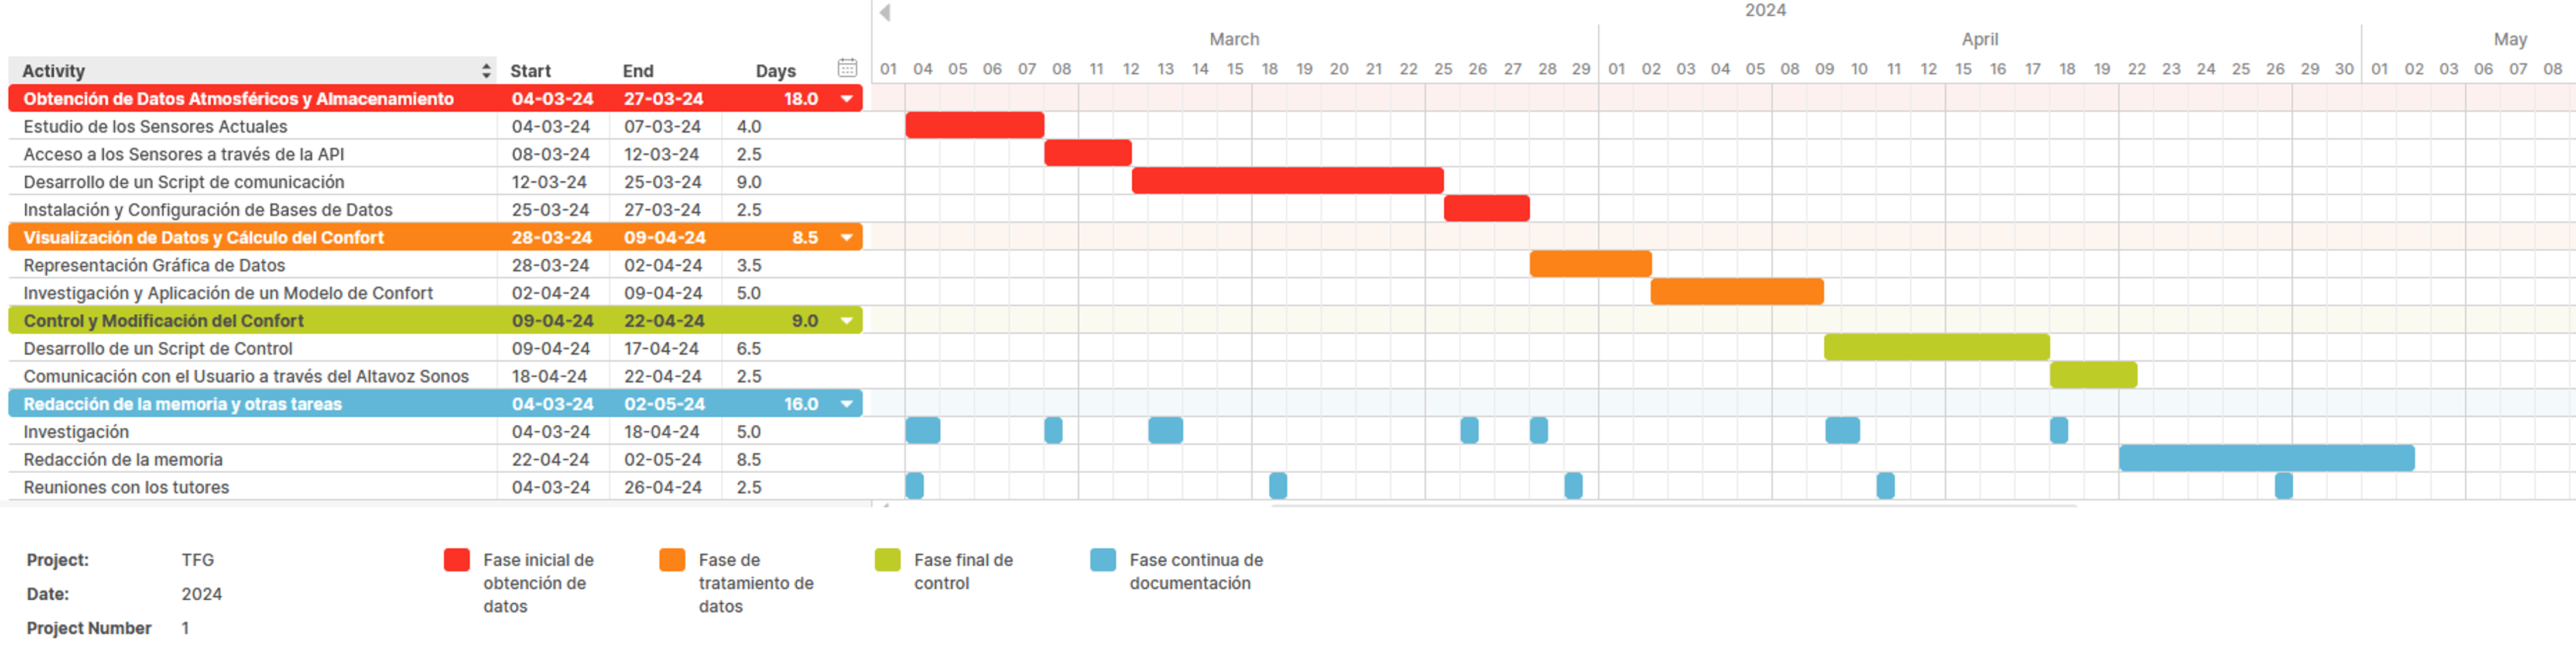
\includegraphics[width=16cm]{Imágenes/Capítulo 1/Ilustración 3. Planificación temporal.png}
        \caption{Planificación Temporal del TFG}
        \label{fig:planificacion_temporal_TFG}
    \end{figure}

\section{Estructura del documento}

El contenido del trabajo se divide en los siguientes capítulos:

\begin{itemize}
    \item \textbf{Introducción:} es la sección actual, donde se realiza una introducción y se explican los objetivos y estructura del trabajo.
    \item \textbf{Capítulo 1. Contexto del trabajo, justificación y motivación:} en este capítulo se describirán las herramientas usadas y las características de la \textit{Smarthome}.
    \item \textbf{Capítulo 2. \textit{API} y \textit{Endpoints} de la \textit{Smarthome}:} en este capítulo se tratará el acceso a los sensores de la \textit{Smarthome}, utilizando la \textit{API} de su servidor y los \textit{endpoints} que ofrece, a través de un \textit{script} en \textit{Python}.
    \item \textbf{Capítulo 3. Almacenamiento en Bases de Datos de los datos recogidos:} en este capítulo se explica cómo almacenar en las distintas bases de datos todos los datos recogidos por las sensores, a través del \textit{script} evolucionado.
    \item \textbf{Capítulo 4. Visualización de los datos en \textit{Grafana}:} en este capítulo se mostrará la interfaz de \textit{Grafana} diseñada, junto a los gráficos con los datos recatados de las bases de datos, para la revisión de la \textit{Smarthome}.
    \item \textbf{Capítulo 5. Cálculo y monitorización del Confort de la \textit{Smarthome}:} en este capítulo se estudiarán los distintos métodos de cálculo de confort y se propondrá el método elegido para este trabajo.
    \item \textbf{Capítulo 6. Control y modificación del Confort:} en este capítulo se desarrollarán los criterios elegidos para actuar sobre diferentes elementos de la \textit{Smarthome} y conseguir alcanzar un Confort óptimo, a través de la siguiente evolución del \textit{script}.
    \item \textbf{Conclusiones y mejoras:} en esta sección se plantearán tanto las conclusiones del trabajo realizado como aquellos aspectos en los que mejorar y continuar el trabajo.
\end{itemize}

%
 \chapter{Apartados del CUERPO DEL DOCUMENTO}

El llamado ``cuerpo del documento'' es el grupo de apartados donde se describe como  se ha desarrollado el trabajo. En el dominio de la Informática, un TFG debe mantener un equilibrio entre la componente de investigación y la componente puramente técnica asociada con el proyecto de desarrollo de software. Un projecto software conlleva la elaboración de una serie de memorias, cada una recopilando lo hecho a distintos niveles, ver figura \ref{fig:report}. Sin embargo la memoria de un TFG es de carácter académico y ademas de artefactos, presupuestos y modelos debe incluir determinadas cuestiones que muestren como se han desarrollado las ideas propias. El punto de partida es la estructura típica de un articulo que se muestra en la figura \ref{fig:articulo}.


\begin{figure}

	\begin{center}
		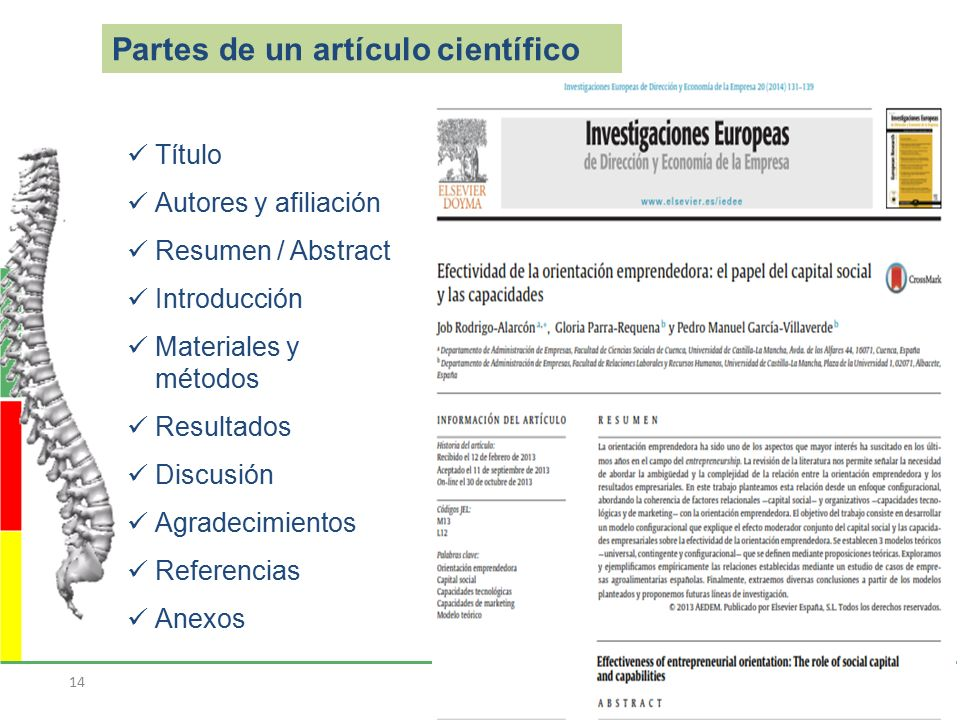
\includegraphics[scale = 0.45]{Figuras/articulo.jpg}
	\end{center}
	\caption{Estructura clásica de un articulo de investigación}
	\label{fig:articulo}
\end{figure}


\begin{figure}  
 	\begin{center}
        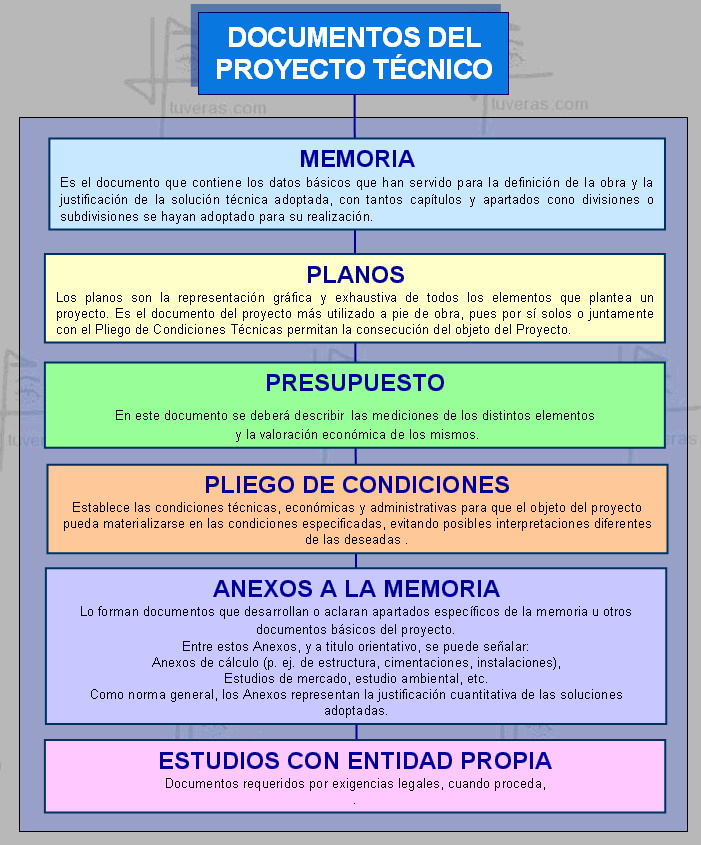
\includegraphics[scale = 0.45]{Figuras/documentos.jpg}
        	\end{center}
        \caption{Estructura de documentos de un proyecto técnico}
    \label{fig:report}
\end{figure}


La propuesta de estructura se define a continuación indicando que se incluiría en cada apartado. Lo importante en este caso es \textsc{que hay que incluir} la estructura del TFG final de cada alumno puede ser diferente, uniendo o separando los contenidos que se detallan a continuación. 

\paragraph{Objetivos o cuestiones de investigación}

se establecerá el objetivo general y los específicos, es decir, cuestiones que serán respondidas con el trabajo que se va a realizar. No es
imprescindible elaborar un apartado específico denominado OBJETIVOS, pues éstos puede quedar reflejados al final de la
introducción

\paragraph{Planificación temporal} 
Se debe incluir una referencia a como se han distribuido las tareas a lo largo del tiempo empleado en el TFG. Esta cuestión deriva de los proyectos técnicos de disciplinas de ingeniería. Puede representarse en forma de tabla o gráfico \ref{fig:plan} y puede aparecer dentro del apartado de metodología.



\begin{figure} 
\begin{ganttchart}[
hgrid,
vgrid={*6{draw=none},dotted},
x unit=0.5mm,
y unit title =0.6cm,
y unit  chart=1cm,
canvas/.style={draw=none},
%title/.append style={fill=black!10, rounded corners=1mm},
title/.append style={ rounded corners=0.5mm},
time slot format=isodate,
time slot format/base century=2000,
time slot unit= day,
time slot format/start date=2020-11-25,
bar height=0.5,
 bar label node/.append style={left=0.01cm, align=left, text width=8em},
 bar label text={$\star$#1},
 bar label font=\sffamily\footnotesize,
 group label node/.append style={left=0.01cm, align=left, text width=8em},
  group peaks width={3},
   group label font=\bfseries\footnotesize,
milestone label font=\scshape\sffamily\footnotesize,
  milestone inline label node/.append style={left=5mm},
  milestone right shift=2,
    milestone left shift=-2,
 milestone/.append style={fill=black!40}
]{2020-11-24}{2021-06-30}
\gantttitlecalendar[y unit title=0.7cm, title height=0.6]{year, month=shortname ,week} \\

\ganttgroup[ bar height=.1]{Selección área}{2020-11-24}{2020-11-30} \\
\ganttbar[name=b2]{Envío de Correos de contacto}{2020-11-24}{2020-11-26}\\
\ganttbar[name=b2]{Realizar Entrevistas}{2020-11-27}{2020-11-30}\\
\ganttmilestone{Área y tutor definido}{2020-11-30} \\ %\ganttnewline
\ganttgroup[bar height=.1]{Estudio preliminar}{2020-12-01}{2020-12-22}\\
\ganttlinkedbar{Task 2}{2020-12-01}{2020-12-22} \\
\ganttbar{Final Task}{2020-12-01}{2020-12-22}\\
\ganttbar{Task 2}{2020-12-01}{2020-12-22}
%\ganttlink{elem2}{elem3}
%\ganttlink{elem3}{elem4}
\end{ganttchart}
        \caption{Planificación del proyecto sobre latex}
    \label{fig:planb}
\end{figure}


\begin{figure}  
 	\begin{center}
        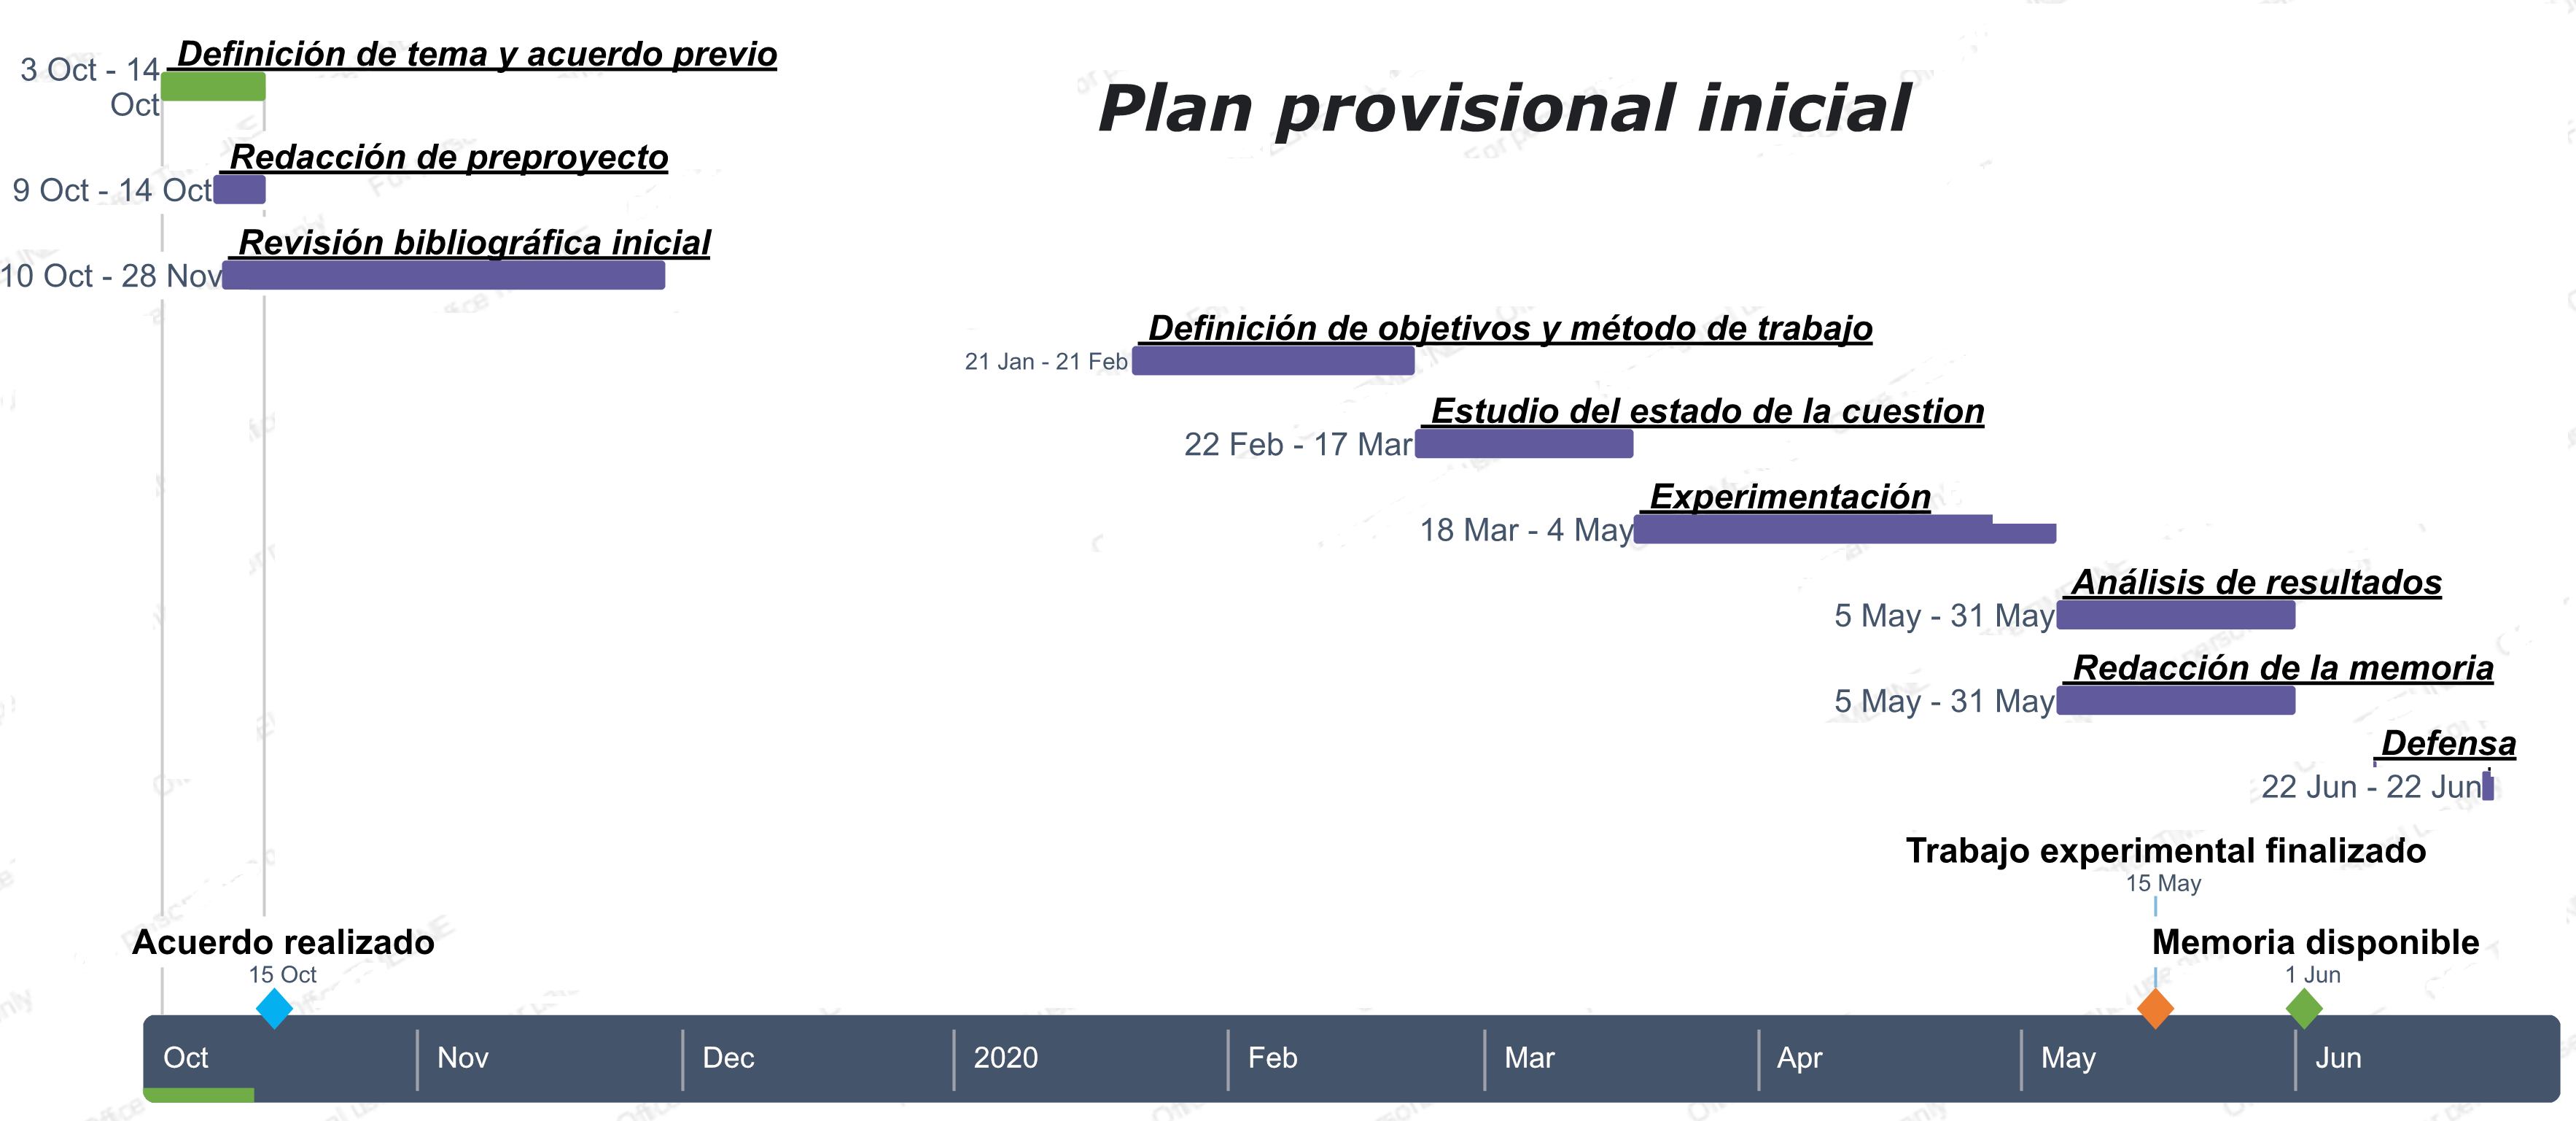
\includegraphics[width=0.8\textwidth]{Figuras/plandef.png}
        	\end{center}
        \caption{Planificación del proyecto}
    \label{fig:plan}
\end{figure}

\paragraph{Contextualización o estado del arte}

Se hará mención a los elementos conceptuales que  sirven  de  base  para  la  investigación,  estudios  previos  relacionados  con  el problema planteado, etc. En este apartado es importante hacer un estudio de los trabajos previos o revisión bibliográfica \cite{kitchenham2009systematic,kitchenham_2013}. Si como es habitual se tiene  que utilizar una o varias herramientas software es en este apartado donde se recogen las alternativas consideradas y cual de ellas ha sido elegida  y porqué.

\paragraph{Metodología}
¿Qué procedimiento se ha seguido para alcanzar los objetivos
planteados? Se  indicará  el  tipo  o  tipos  de  investigación,  las  técnicas  y  los procedimientos  que  serán  utilizados  para  llevarla  a  cabo;  se  identificará la población  y  el  tamaño  de  la  muestra  así  como  las técnicas  e  instrumentos  de recolección de datos, si te trata de un trabajo empírico, la metodología de desarrollo de software seleccionada. O cualquier otra información sobre el proceso seguido. La planificación y objetivos también pueden estar en este apartado

 
\paragraph{Resultados}
Incluirá  los  resultados  de  la  investigación  o  trabajo,  así como el análisis y la discusión de los mismos, aunque algunos tutores prefieren dos apartados separados. En el caso de tratarse de un desarrollo de software en este apartado se incluirá la descripción del producto resultante y los modelos o artefactos softtware necesarios para su descripción. Pero el manual o tutorial detallado  y los modelos completos deberían llevarse a los anexos.


La discusión conlleva revisar que aporta el trabajo realizado y se  han conseguido los objetivos planteados inicialmente. Caso de tener una evaluación por parte de los clientes potenciales también aparecerá en este apartado.


 \chapter{Apartado BIBLIOGRAFIA}
 Este apartado es de vital importancia para tener éxito en la consecución del trabajo fin de grado. Los tribunales suelen prestar gran atención a este apartado, probablemente por su formación académica. 
 
 Es todo un mundo el de los estilos bibliográficos y la realización de las citas, se puede encontrar un tutorial en:  \url{http://ci2.ual.es/comunicar-la-informacion/citas-y-referencias-bibliograficas/}. No obstante en las siguientes secciones se indicarán las cuestiones básicas para iniciarse en el tema pero restringuiendose a la utilización de la presente plantilla. La gran ventaja de latex es que cada elemento en las referencias   \lstinline[language=enparrafo]!\bibitem! es considerado como un elemento de una base de datos, de forma que es el compilador el que reordena o coloca la cita de acuerdo con el estilo definido.

 \section{Como citar}
A lo largo del texto de la memoria se incluirán citas a trabajos de otros autores. La inclusión de la cita tiene que ser justo después del texto donde se propone algo relativo al trabajo citado. Para citar, como para todo el \LaTeX{} existen numerosos paquetes, los dos mas conocidos son  biblatex y   natbib . 

Además dada forma de citar y de incorporar items en el apartado referencias lleva asociado un estilo de bibliografía    \lstinline[language=enparrafo]!\bibliographystyle{XXX}!, que aun abre mucho mas el abanico de opciones. 

Es recomendable consultar las ayudas de los paquetes \url{https://www.overleaf.com/learn/latex/Biblatex_bibliography_styles} y \url{https://www.overleaf.com/learn/latex/Bibliography_management_with_natbib}.

Lo habitual es utilizar la orden      \lstinline[language=enparrafo]!\cite{xxx}!, o   \lstinline[language=enparrafo]!\citep(xxx)!  en la ubicación en el texto donde se quiere colocar la cita, el compilador se encargá de procesarla según el estilo.

 \section {Apartado referencias}
  Existen dos formas de incorporar las referencias, directamente en el entorno   \lstinline[language=enparrafo]!\begin{bibliography}! y utilizando las ordenes del lenguaje o bien utilizando un archivo .bib para guardar esas referencias. Se generará un auxiliar .bbl que automáticamente se incorpora en el documento.
  
  Este archivo auxiliar es el que tiene directamente las ordenes del lenguaje.
  
 \begin{verbatim}
  
\begin{thebibliography}{3}

\bibitem{SWEBOK2014}
P.~Bourque and R.~E. Fairley, Eds., \emph{{SWEBOK}: Guide to the Software
  Engineering Body of Knowledge}, version 3.0~ed.\hskip 1em plus 0.5em minus
  0.4em\relax Los Alamitos, CA: IEEE Computer Society, 2014.

\bibitem{kitchenham_2013}
B.~Kitchenham and P.~Brereton, ``A systematic review of systematic review
  process research in software engineering,'' \emph{Information and Software
  Technology}, vol.~55, no.~12, pp. 2049 -- 2075, 2013.

\bibitem{basili1992}
V.~R. Basili, ``Software modeling and measurement: the goal/question/metric
  paradigm. cs-tr-2956, umiacs-tr-92-96,'' University of Maryland, Tech. Rep.,
  1992.
\end{thebibliography}

  \end{verbatim}
 
 
 
 \section{Archivos .bib}
 
 BibTeX, y natbib por extensión, usan un archivo externo en texto plano como base de datos de referencias bibliográficas para generar las bibliografías y sus referencias en documentos con distintos formatos de artículos, libros, tesis, presentaciones, etc. Los nombres de archivos de referencias bibliográficas de BibTeX usualmente terminan o usan la extensión .bib. Los ítems bibliográficos incluidos en un .bib están separados por tipos.
 
 \begin{verbatim}
@inbook{Berander2005,
        address = {Berlin, Heidelberg},
        author = {Berander, Patrik and Andrews, Anneliese},
        booktitle = {Engineering and Managing Software Requirements},
        pages = {69--94},
        publisher = {Springer Berlin Heidelberg},
        title = {{Requirements Prioritization}},
        doi= {https://doi.org/10.1007/3-540-28244-0{\_}4},
        year = {2005}
} 
 \end{verbatim}
 
 Los tipos que son reconocidos por virtualmente todos los estilos de BibTeX se muestran en el anexo \ref{sec:bib}. Pero igual que antes es recomendable recurrir a tutoriales o recursos donde se describan con detalle. Además se recomienda la utilización de algún gestor de referencias bibliográficas tipo Mendeley. \url{https://www.mendeley.com/}


\addcontentsline{toc}{section}{BIBLIOGRAFÍA }
\bibliography{referencias}

\appendix
%\clearpage


\addtocontents{toc}{ \vspace{5mm} \hrule \par}


\chapter {Contenido de una entrada en .bib}
\begin{table} 
	\begin{center}
	\begin{tabular}{l p{10cm} }
		\textbf{Nombre campo} & \textbf{Descripción} \\ \hline

address&Usualmente la dirección de la editorial\\
author&Nombre(s) del (de los) autor(es)\\
title&Título del libro\\
chapter&El número de un capítulo (o sección, etc)\\
edition&La edición de un libro, por ejemplo,segunda\\
editor&Nombre(s) del (de los) editor(es)\\
howpublished&Forma en que fue publicada la obra\\
institution&Institución responsable de un informe técnico\\
journal&Nombre del periódico o revista\\
key&Empleado para la alfabetización, referencias cruzadas y para crear una clave cuando la información del autor no está disponible. No debe confundirse con la etiqueta usada en el cite y que debe colocarse al inicio de la entrada\\
month&El mes de publicación o, para un trabajo inédito, en el que fue escrito\\
note&Cualquier información adicional que pueda ayudar al lector\\
number&El número del periódico, la revista, el informe técnico o del trabajo en una serie\\
organization&La organización responsable de una conferencia o que publica un manual\\
pages&Números de páginas\\
publisher&El nombre de la editorial. No debe confundirse con el editor\\
school&Nombre de la escuela donde fue escrita una tesis\\
series&El nombre de una serie o conjunto de libros\\
title&El título del trabajo\\
type&El tipo de un informe técnico\\
volume&El volumen de un periódico o una revista, o de algún libro que conste de volúmenes\\
year&El año de publicación. Para un trabajo inédito, el año en que fue escrito. Generalmente debe consistir de cuatro dígitos, por ejemplo 200\\
         \hline
	\end{tabular}
	\end{center}
	\caption{Campos de una entrada en archivo de bibliografía .bib}
\end{table}



  \chapter{Tipos de referencias}
  \label{sec:bib}
    \begin{table} 
	\begin{center}
	\begin{tabular}{l p{10cm} }
	 \hline
   article& Un artículo de un periódico o revista\\
  
    book& Un libro con una editorial que se indica en forma explícita. Los campos requeridos en este caso son author (autor), editor, title (título), publisher (editorial) y year (año)\\
  
    booklet& Una obra que está impresa y encuadernada, pero sin una editorial o institución patrocinadora\\
  
    conference& Lo mismo que inproceedings, incluido para compatibilidad con el lenguaje de marcación Scribe\\
  
    inbook& Una parte de un libro, que puede ser un capítulo (o sección) o un rango de páginas\\
  
    incollection& Una parte de un libro que tiene su propio título\\
  
    inproceedings& Un artículo en las actas de sesiones (proceedings) de una conferencia\\
  
    manual& Documentación técnica\\
  
    mastersthesis& Una tesis de maestría (Master thesis) o proyecto fin de carrera\\
  
    misc& Para uso cuando los demás tipos no corresponden\\
  
    phdthesis& Una tesis de doctorado (Ph D thesis)\\
  
    proceedings& Las actas de sesiones de una conferencia\\
  
    techreport& Un reporte publicado por una escuela u otra institución, usualmente numerado dentro de una serie\\
  
    unpublished& Un documento que tiene un autor y título, pero que no fue formalmente publicado\\
          \hline
	\end{tabular}
	\end{center}
	\caption{Tipos posibles de elementos en bibligrafía con natbib}
\end{table}

 
  \chapter *{Artefactos software}






\clearpage
\backmatter

\thispagestyle{empty}
%\put(0,0){
\begin{minipage}[h]{0.9\paperwidth}
\thispagestyle{empty}
\begin{tikzpicture}[remember picture,overlay]
\node (f) [rectangle]  
at (current page.center)
          {\parbox[b][\paperheight]{\paperwidth}{
           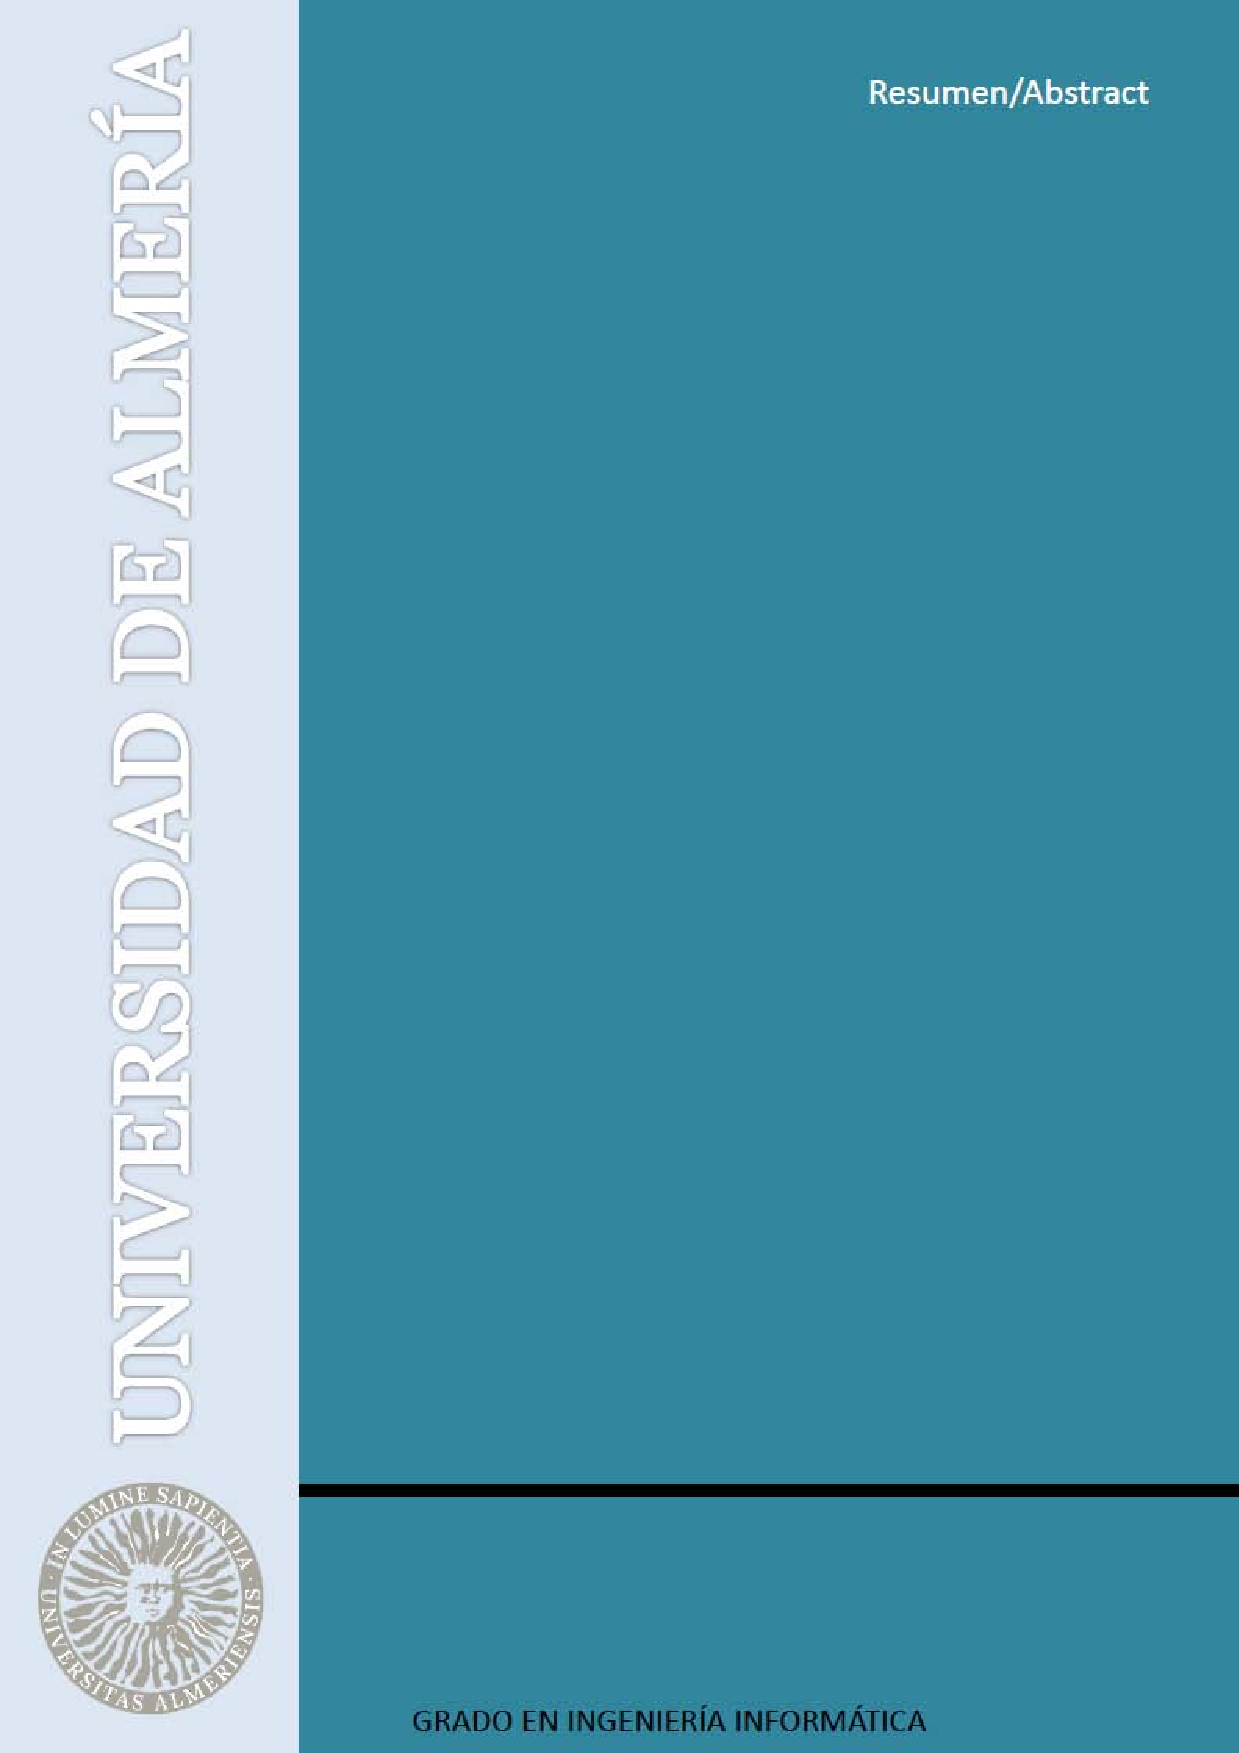
\includegraphics[width=\paperwidth,height=\paperheight,keepaspectratio]{Figuras/logos/TFG_back}
          }};
\node (texto) [rectangle,text width=0.5\paperwidth,yshift=150pt] 
at (f)
          {\parbox{0.65\paperwidth}{\justifying \Large \color{white}
         En este archivo se incluirá tanto el resumen en castellano como su traducción al inglés. Los dos párrafos estarán ligeramente separados.

El  propósito  del  trabajo  en  una  o  dos  frases.  El  diseño  y metodología  utilizada,  los  resultados  más  significativos  del trabajo realizado y un breve resumen de las conclusiones. Debe ser conciso y presentar los resultados obtenidos tras la ejecución del TFG. 

\vspace{1.5cm}

%\section*{Abstract}
Put here  the english tranlation  ... . Debe ser conciso y presentar los resultados obtenidos tras la ejecución del TFG. Los dos parrafos estarán ligeramente separados.
         }};
       \node  at (14,-25.55) {\Large\curso};
  \end{tikzpicture}
\end{minipage}
%}


          
          

\end{document}
